\begin{figure}[tbp]
\centering
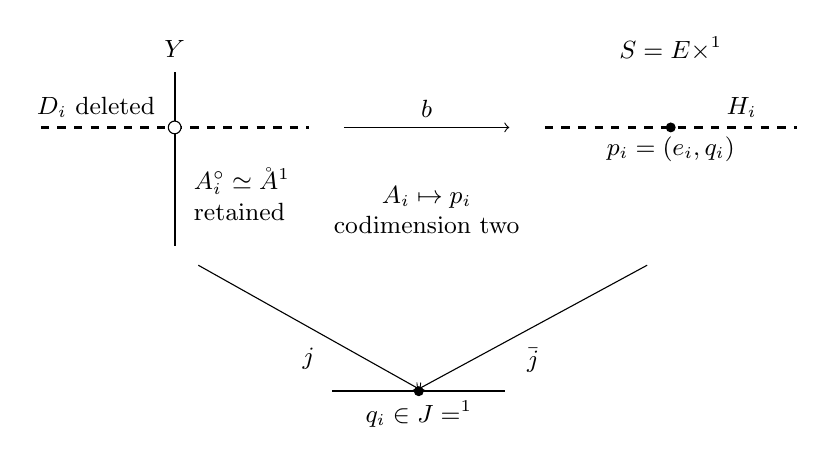
\begin{tikzpicture}[x=1cm,y=1cm,font=\small]
  \node at (0,2) {$Y$};
  \draw[dashed,thick] (-1.7,1)--(1.7,1);
  \node[above] at (-1,1) {$D_i$ deleted};
  \draw[thick] (0,-.5)--(0,1.7);
  \filldraw[fill=white] (0,1) circle (2.3pt);
  \node[right,align=left] at (.12,.15)
    {$A_i^\circ\simeq\AA^1$\\retained};
  \draw[->] (2.15,1)--(4.25,1) node[midway,above] {$b$};
  \node[align=center] at (3.2,-.05)
    {$A_i\mapsto p_i$\\codimension two};
  \node at (6.3,2) {$S=E\times\PP^1$};
  \draw[dashed,thick] (4.7,1)--(7.9,1);
  \fill (6.3,1) circle (1.8pt);
  \node[above] at (7.2,1) {$H_i$};
  \node[below] at (6.3,1) {$p_i=(e_i,q_i)$};
  \draw[->] (.3,-.75)--(3.1,-2.32)
    node[midway,below=4pt] {$j$};
  \draw[->] (6,-.75)--(3.1,-2.32)
    node[midway,below=4pt] {$\bar j$};
  \draw[thick] (2,-2.35)--(4.2,-2.35);
  \fill (3.1,-2.35) circle (1.8pt);
  \node[below] at (3.1,-2.35) {$q_i\in J=\PP^1$};
\end{tikzpicture}
\smallskip
\[
\begin{array}{c|c|c}
 & \text{multiplicity at }q_i & \text{boundary coefficient}\\ \hline
\text{direct base} & \min\{\infty,1\}=1 & 0\\
\text{iterated base} & \infty & 1
\end{array}
\]
\caption{Incidence schematic showing the two routes to the same point
$q_i$. The horizontal arrow is
the blowdown of complete surfaces: the retained $A_i^\circ$ maps to a
point on $H_i$. The hollow point $A_i\cap D_i$ is removed from $X$.
The divisor $A_i$ is omitted from the intermediate orbifold base because
$b(A_i)$ has codimension two in $S$, but contributes multiplicity one
to the direct base over $q_i$.}
\label{fig:retained-exceptional}
\end{figure}
